% ELEC2302 Lecture 4 — "Approximating a periodic signal".
%   (a) least-squares approximation of one vector by another in the plane:
%       the projection c*phi, with the error u - c*phi perpendicular to phi.
%   (b) the same construction for signals: a square wave of period 2 pi and
%       the best approximation by a single sinusoid at the fundamental,
%       (4/pi) cos(omega t).
% House style: navy #00468C for u, brick #C0392B for the approximation.
%
% Build:
%   latex projection.tex && dvisvgm --no-fonts --exact -o projection.svg projection.dvi
%
\documentclass[tikz,border=3pt,dvisvgm]{standalone}
\usepackage{amsmath}
\usepackage{pgfplots}
\pgfplotsset{compat=1.18}
\usetikzlibrary{arrows.meta, calc, positioning}

\definecolor{navy}{HTML}{00468C}
\definecolor{brick}{HTML}{C0392B}
\definecolor{ash}{HTML}{8A8A8A}
\definecolor{mist}{HTML}{C9C9D0}

\begin{document}
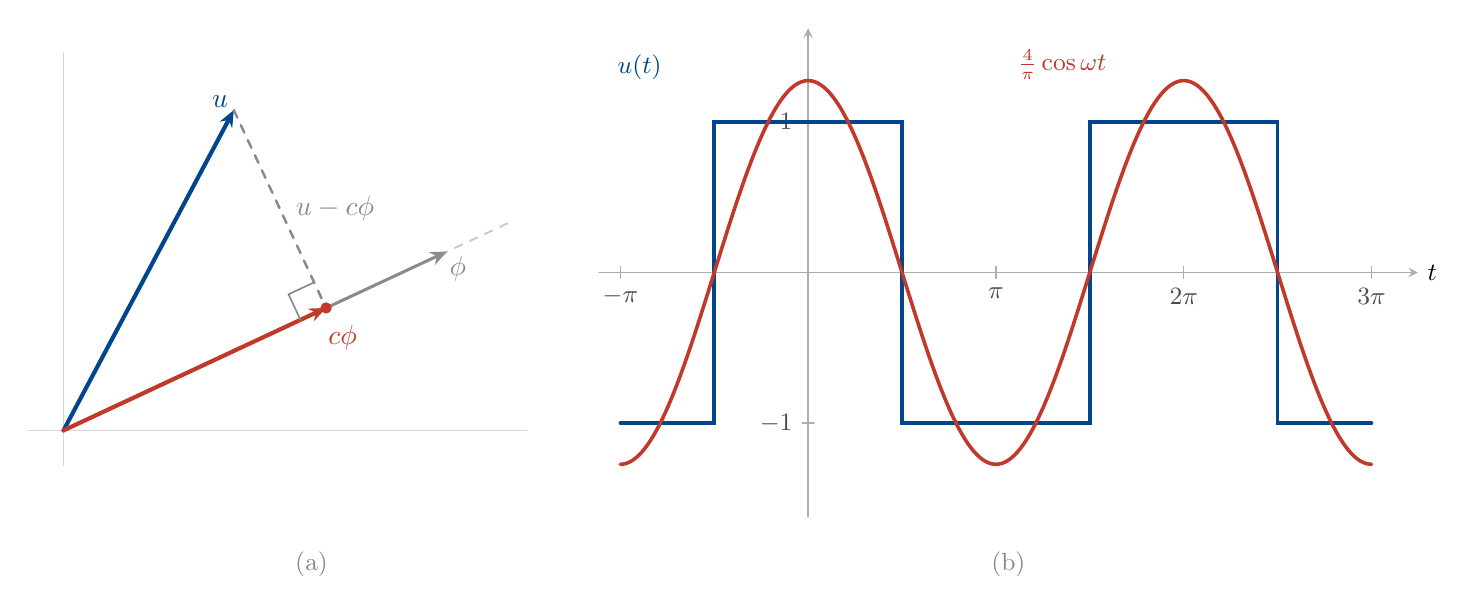
\begin{tikzpicture}[>={Stealth[length=6pt,width=5pt]}, line cap=round]

% ============================== (a) projection in the plane
% phi at 25 degrees, u at 62 degrees; c phi is the foot of the perpendicular
% from the tip of u onto the line spanned by phi.
\begin{scope}[scale=1.28, yshift=-0.2cm]
  % a hint of the plane, kept faint: the construction does not use coordinates
  \draw[ash!35, line width=0.4pt] (-0.35,0) -- (4.60,0);
  \draw[ash!35, line width=0.4pt] (0,-0.35) -- (0,3.75);

  % the line spanned by phi
  \draw[mist, line width=0.7pt, dashed] (0,0) -- (4.45,2.075);

  % phi, u, and the projection c phi
  \draw[ash, ->, line width=1.1pt] (0,0) -- (3.806,1.775) node[below right=-2pt and -3pt] {$\phi$};
  \draw[navy, ->, line width=1.5pt] (0,0) -- (1.690,3.178) node[above left=-3pt and -2pt] {$u$};
  \draw[brick, ->, line width=1.5pt] (0,0) -- (2.605,1.215) node[below=2pt, xshift=6pt] {$c\phi$};

  % the error, perpendicular to phi
  \draw[ash, dashed, line width=0.9pt] (1.690,3.178) -- (2.605,1.215)
        node[midway, right=2pt] {$u - c\phi$};

  % right angle at the foot of the perpendicular
  \draw[ash, line width=0.6pt]
        ($(2.605,1.215)+(25:-0.28)$) -- ++(115:0.28) -- ++(25:0.28);

  \fill[brick] (2.605,1.215) circle (1.6pt);
\end{scope}

% ============================== (b) square wave and its fundamental
\begin{scope}[xshift=12.0cm, yshift=1.75cm]
  \begin{axis}[
      width=10.4cm, height=6.2cm,
      scale only axis,
      at={(0cm,0cm)}, anchor=center,
      axis lines=middle,
      axis line style={ash!70, line width=0.5pt},
      xmin=-3.5, xmax=10.2, ymin=-1.62, ymax=1.62,
      xtick={-3.14159, 0, 3.14159, 6.28319, 9.42478},
      xticklabels={$-\pi$, , $\pi$, $2\pi$, $3\pi$},
      ytick={-1,1}, yticklabels={$-1$,$1$},
      tick style={ash!70, line width=0.5pt},
      tick label style={font=\small, color=black!70},
      xlabel={$t$}, xlabel style={at={(axis description cs:1.0,0.5)}, anchor=west, font=\small},
      clip=false,
    ]
    % the square wave u(t): +1 around t = 0, period 2 pi
    \addplot[navy, line width=1.3pt] coordinates {
      (-3.14159,-1) (-1.570796,-1) (-1.570796,1) (1.570796,1) (1.570796,-1)
      (4.712389,-1) (4.712389,1) (7.853982,1) (7.853982,-1) (9.42478,-1)
    };
    % the best approximation by a single sinusoid at the fundamental
    \addplot[brick, line width=1.3pt, samples=300, domain=-3.14159:9.42478]
      {4/pi*cos(deg(x))};

    \node[navy, font=\small, anchor=west] at (axis cs:-3.35,1.36) {$u(t)$};
    \node[brick, font=\small, anchor=west] at (axis cs:3.35,1.38) {$\tfrac{4}{\pi}\cos\omega t$};
  \end{axis}
\end{scope}

% ============================== panel labels, on a common baseline
\node[ash, font=\small] at (3.15cm,-1.95cm) {(a)};
\node[ash, font=\small] at (12.0cm,-1.95cm) {(b)};

\end{tikzpicture}
\end{document}
